
\section{Structure on \texorpdfstring{$K$}{K}-theory} % <<<
\label{StructureOnKtheory}
\ifx\OutputStructureOnKtheory\undefined\else
This isn't a course about $K$-theory, it's a course that uses $K$-theory.  So we're not going to see proofs of lots of basic theorems of $K$-theory; in particular I'm not going to prove the periodicity theorem.  However, we will need some facts which we'll review now.

Recall that we previously defined the group $\KOtwee(X)$, and by doing the same constructions using complex vector bundles we get $\Ktwee(X)$.  Let's see what $\Ktwee S^2$ is.  $S^2$ splits into contractible hemispheres $D_\pm$ over which any vector bundle is trivial, $D_\pm \times \C^n$.  The construction of a vector bundle on $S^2$ therefore amounts to choosing over each point on the equator $S^1$ a linear isomorphism $\C^n \to \C^n$ in a continuous manner, i.e., a map $S^1 \to GL_n(\C)$.  So, $\Vect_{n,\C}(S^2) \cong \pi_1 GL_n(\C)$.  This way of constructing vector bundles is called the ``clutching construction.''  There are compatible deformation retractions
%
\begin{ctikzcd}
\cdots\rar[hook] & GL_n(\C)\rar[hook]\dar &GL_{n+1}(\C)\rar[hook]\dar&\cdots\\
\cdots\rar[hook] & U(n)\rar[hook]&U(n+1)\rar[hook]&\cdots\\
\end{ctikzcd}
%
and hence we may assume all our maps have codomain $U(n)$ instead.\footnote{The existence of such a retract implies that there is a functorial way to assign Hermitian inner products to complex vector bundles.}  Each inclusion on the bottom row occurs as the fiber of a bundle\footnote{Note that $U(n+1)$ acts on $S^{2n+1}$. Choosing a basepoint $b\in S^{2n+1}$, the map $U(n+1)\to S^{2n+1}$ given by $x\mapsto xb$ is a fibration with fiber the stabiliser of $b$. Of course, the stabiliser is $U(n)$.} $U(n+1) \to S^{2n+1}$, and hence we calculate using the long exact sequence of homotopy groups that $\pi_1 U(n) \cong \pi_1 U(n+1)$ induced by these inclusions for $n \ge 1$. In particular, $\pi_1 U(1) \cong \pi_1 S^1 = \Z$, so that $\pi_1 U(n)\simeq \Z$, where homotopy class corresponding to $k\in \Z$ is that of the map $z\mapsto\textup{diag}(z^k,1,1,\ldots)$ for $z\in S^1=U(1)$.

Now if $V_{n,k}$ is the $n$-dimensional complex bundle obtained by clutching along the element of $\pi_1 U(n)$ corresponding to $k\in\Z$, it is not hard to see that $V_{n,k}\oplus V_{n',k'}$ is isomorphic to $V_{n+n',k+k'}$. From this we see that $\Ktwee(S^2) \cong \Z$, generated by $[V_{1,1}]-1$.

Now we have represented the generator of $\pi_1 U(1)$ as the identity, which as a clutching function represents $\bundle{L} \onto \CP^1 \simeq S^2$, the tautological (complex) line bundle.  Hence, a generator of $\Ktwee S^2$ is $[\bundle L] - 1$.  Similarly, since all the unitary groups are connected, $\Ktwee(S^1) = 0$.

\begin{fact}
In the real case, we have $\KOtwee(S^8) = \Z$, generated by the tautological Cayley $\mathbb{H}$-line bundle, considered as a 4-dimensional real bundle over $\mathbb{H}P^2 \simeq S^8$. (What happens if we use octonions?) % is this last bit right?  and what about the octonions?
\end{fact}

\begin{thm}[Bott periodicity]
\begin{align*}
\Ktwee (X) \otimes \Ktwee (S^2) & \stackrel{\cong}{\to} \Ktwee(X \sprod S^2) \\
\KOtwee (X) \otimes \KOtwee (S^8) & \stackrel{\cong}{\to} \KOtwee(X \sprod S^8).
\end{align*}
\end{thm}

A word on this tensor product: an element of $\Ktwee (X)$ is a ``virtual vector bundle'' $V - m$, where $m$ is the trivial bundle of dimension $m = \dim V$.  If $V - m \in \Ktwee(X)$ and $W - n \in \Ktwee(S^2)$, then we define earlier their exterior tensor product over $X \times S^2$ in the obvious way: $(V - m)\hat\otimes(W - n) = V \hat\otimes W - m \hat\otimes W - V \hat\otimes n + m \hat\otimes n$.  Consider now what this bundle looks like over $X \vee S^2 \subseteq X \times S^2$: on $X \times \ptspace$, $W$ is trivial, so we get $V \hat\otimes n - m \hat\otimes n - V \hat\otimes n + m \hat\otimes n = 0$; on $\ptspace \times S^2$ we see that $V$ is trivial, so we get $m \hat\otimes W - m \hat\otimes W - m \hat\otimes n + m \hat\otimes n = 0$.  Hence, the bundle $(V - m) \hat\otimes (W - n)$ is trivial over $X \wsum S^2$, and so pulls back from a vector bundle over $X \sprod S^2$.  This at least exhibits the map above.

Next let's see how the periodicity theorem can be used to make $KO$ and $K$ the $0^\textup{th}$ groups of periodic generalized cohomology theories with periods $8$ and $2$ respectively.  The first thing we observe is that $\KOtwee$ is representable; recall that $\KOtwee(X)$ is given by pointed homotopy classes of maps $X \to BO \times \Z$, denoted $[X, BO \times \Z]$ (we'll start writing $B$ for $BO \times \Z$).  Cued by the suspension isomorphism from singular cohomology, for $n \ge 0$ we define:
\begin{align*}
\qquad\qquad\qquad
\KOtwee^{-n} (X) & = \KOtwee(\Suspend^n X)\hbox{\ for $n\geq0$}, \\
\KOtwee^n(X) & = \KOtwee(\Suspend^{8k-n}X) \hbox{\ for any $k$ with $8k > n$}, \\
KO^*(X) &= \KOtwee^* X_+, \\
KO^*(X, A) & = \KOtwee^*(X \cup CA) \textup{\ when $A\hookrightarrow X$ is a cofibration.}
\end{align*}

For this to be considered a cohomology theory we need some long exact sequences.  Now its a general fact that for a map of pointed spaces $f: A \to X$ if we take the mapping cone $A \stackrel{f}{\to} X \to X \cup_f CA = C(f)$, then the sequence
\[
[A, B] \from [X, B] \from [X \cup CA, B]
\]
is exact.  Moreover, when $B$ is an $H$-space then the induced homomorphisms of groups are exact.  Now we can continue; that is, take the mapping cone of $X \to X \cup_f CA$:
\[
A \stackrel{f}{\to} X \stackrel{i}{\to} X \cup_f CA \to (X \cup_f CA) \cup_i CX \to \cdots
\]

%\begin{wrapfigure}{r}{0.4\textwidth}
%\centering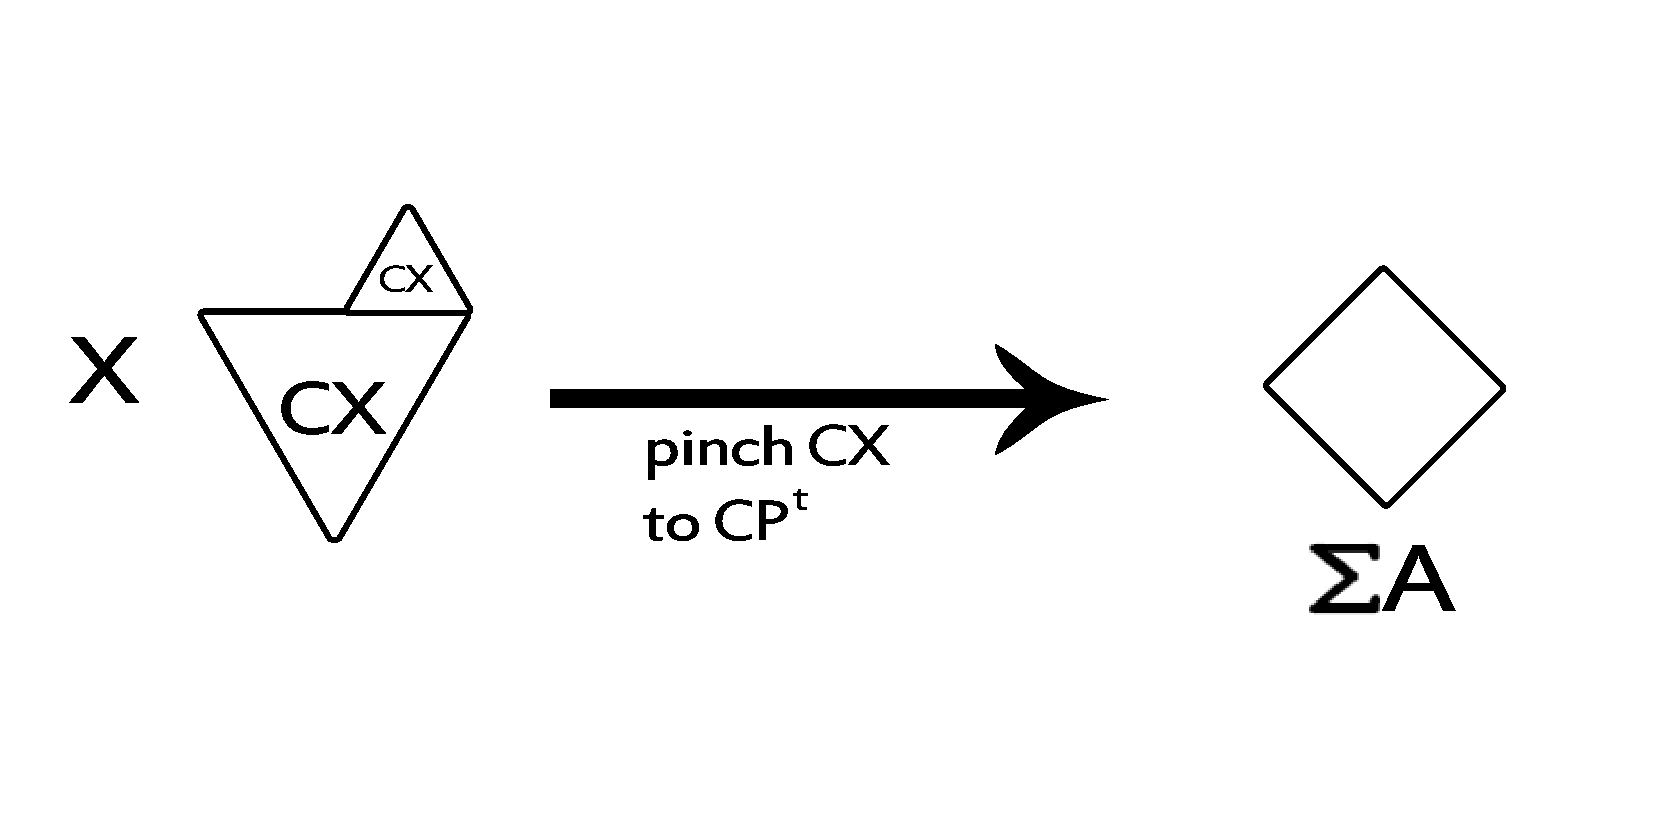
\includegraphics[width=0.3\textwidth]{figures/13.pdf}
%\caption{\small The going-around quotient.}
%\end{wrapfigure}
Now, if $f$ is nice enough, $X \cup CA$ will be homotopic to $X / A$.  Certainly $(X \cup CA) \cup CX \simeq (X \cup CA)/X$, so the sequence becomes
\[
A \to X \to X \cup CA \to \Suspend A \to \Suspend X \to \cdots
,\]
and moreover the map $\Suspend A \to \Suspend X$ can in fact by given by $\Sigma f$ up to homotopy.  This sequence is called the ``Barratt-Puppe'' sequence.  We can then apply the Hom-functor $[-, B]$ to get a long exact sequence\footnote{Applying $[-, Z]$ will give a long exact sequence of pointed sets for any $X$.  Since our $Z = B$ is an $H$-group, this gives a long exact sequence of groups.}
\[
[A, B] \from [X, B] \from [X \cup CA, B] \stackrel{\delta}{\from} [\Suspend A, B] \from [\Suspend X, B] \from \cdots
.\]
Identifying groups as above, we produce a long exact sequence
\[
\KOtwee^0 (A) \from \KOtwee^0(X) \from KO^0(X, A) \from \KOtwee^{-1}(A) \from \KOtwee^{-1}(X) \from \cdots
,\]
and via periodicity we have the full long exact sequence
\[
\cdots \from KO^1(X, A) \from \KOtwee^0 (A) \from \KOtwee^0(X) \from KO^0(X, A) \from \KOtwee^{-1}(A) \from \KOtwee^{-1}(X) \from \cdots
.\]
This justifies our choice of definition of $\KOtwee^*$ above.  This whole setup works similarly for complex $K$-theory.

Now it's an important fact about $\Ktwee^* (X)$ that it's a commutative ring: we calculated $\Ktwee^0 (S^1) = 0$ and $\Ktwee^0 (S^2) = \Z$ with generator $(\bundle{L} - 1)$, which gives a generator $p \in \Ktwee^{-2} (S^0) = K^{-2} (\ptspace)$, called the ``periodicity element.''  So $K^* \eqdef K^* (\ptspace) = \Z[p^{\pm 1}]$, the Laurent series ring, where $|p| = -2$.  Similarly, there is a ring structure for $KO^*$:
\[
\begin{array}{c|ccccccccc}
n & 0 & 1 & 2 & 3 & 4 & 5 & 6 & 7 & 8 \\
\hline
KO^{-n} (\ptspace) & \Z & \Z_2 & \Z_2 & 0 & \Z & 0 & 0 & 0 & \Z \\
\mathrm{generator} & 1 & \eta & \eta^2 & & q & & & & p,
\end{array}
\]
with relations $2\eta = 0$, $\eta^3 = 0$, $\eta q = 0$, $q^2 = 4p$, where $p$ is the periodicity element. For example, $KO^{-10}(\ptspace) = \langle p\eta^2 \rangle \cong \Z_2$ and $KO^{6}(\ptspace) = \langle p^{-1}\eta^2 \rangle \cong \Z_2$, so that $KO^*$ is the ring with generators $\eta,q,p^{\pm1}$ and the given relations.

Unfortunately, we shall need more than just the ring structure; we'll need operations.  One way to get operations in $K$-theory is to look for operations on vector spaces, apply these fiber-wise to get operations on vector bundles, and then squeeze out operations on $K$-theory.  The most useful of these is $V \mapsto \Lambda^k(V)$, the $k$th exterior power.  By means of this method we get a $k^\textup{th}$ exterior power bundle $\Lambda^k E \downarrow B$ from a bundle $E\downarrow B$.  Unfortunately extending to $K$-theory is hard because $\Lambda^k$ is not additive.

There is, however, a natural isomorphism $\Lambda^k(V \oplus W) = \bigoplus_{i+j = k} \Lambda^i V \otimes \Lambda^j W$.  This (which looks like a Cartan formula) inspires the definition $\Lambda_t(V) = \sum_{i \ge 0} t^i \Lambda^i(V)$.  Now $\Lambda_t(V \oplus W) = \Lambda_t(V) \cdot \Lambda_t(W)$, so the operation still isn't additive, but it's exponential --- it takes sums to products.  That's good enough, as it turns out.  So $\Lambda_t$ induces a homomorphism of commutative monoids $\Lambda_t: \Vect(X) \to 1 + t\,KO(X)\llbracket t \rrbracket$, where the target is the group (under multiplication) of formal power series in $t$ with coefficients in $KO(X)$ and constant term one.

By definition of $KO(X)$, there is a group homomorphism $\lambda_t: KO(X) \to 1+t\,KO(X) \llbracket t \rrbracket$ such that the map $\Lambda_t$ factors:
\begin{ctikzcd}
\Vect(X)\rar["\Lambda_t"]\dar & 1+t\,KO(X)\llbracket t \rrbracket\\
KO(X)\urar["\lambda_t"']
\end{ctikzcd}
That $\lambda_t$ is a group homomorphism is to say that
%\[
$\lambda_t(A + B) = \lambda_t(A) \cdot \lambda_t(B)$
%,\]
for $A, B \in KO(X)$. This behaviour is like that of total Steenrod operations.  Of course if $E$ is a vector bundle, then $\lambda^j(E) = \Lambda^j(E) = 0$ for $j > \dim E$ (where $\lambda^j$ is defined, of course, by $\lambda_t(E) = 1 + \sum_{k \ge 1} t^k \lambda^k(E)$.)

The $\lambda$ operations are all very well, but they are hard to work with because they depend on the ring structure of $KO(X)$.  We really want an additive ``power operation,'' so one thing to try is to take a logarithm, in search of a family of operations $\psi^k$ such that on line bundles we get $\psi^k(L) = L^{\otimes k}$.  Once again, we start with a generating function $\psi_t(x) = \sum_{k \ge 1} \psi^k(x) t^k$, then our conditions on $\psi^k$ become:
\begin{align*}
\psi_t(x + y) & = \psi_t (x) + \psi_t (y), \\
\psi_t(L) & = \sum_{k \ge 1} L^k t^k = \frac{Lt}{1 - Lt}.
\end{align*}
The first obvious candidate is \[\log \lambda_t(x) = \sum_{i=0}^\infty (-1)^i \frac{(\lambda_t(x) - 1)^i}{i} = (\lambda_t(x) - 1) - \frac{(\lambda_t(x) - 1)^2}{2} + \frac{(\lambda_t(x) - 1)^3}{3} - \cdots,\] but unfortunately this has denominators,\footnote{Check the $t^2$ coefficient!} and we don't know what $1/n$ means in $KO(X)$.  Our next guess is $\frac{d}{dt} \log \lambda_t(x) = \frac{\frac{d}{dt} \lambda_t(x)}{\lambda_t(x)}$ (and $\lambda_t(x)^{-1}$ exists), and so we have additivity, the first property.  Now for $L$ a line bundle,
\[
\frac{d}{dt} \log (1 + tL) = \frac{L}{1 + tL}
.\]
Replace $t$ with $-t$ to get $\frac{d}{dt} \log(1 - tL) = \frac{-L}{1 - tL}$.  And, to normalize, multiply by $-t$ to get $\frac{tL}{1 - tL} = \sum_{k \ge 1}^\infty t^k L^k$.  We define the $k^\textup{th}$ ``Adams operation'' applied to $E$, $\psi^k(E)$, to be the coefficient of $t^k$ in \[\frac{-t \frac{d}{dt} \lambda_{-t}(E)}{\lambda_{-t}(E)}.\]
Of course, this construction could be carried out on $K(X)$ as opposed to $KO(X)$.

We seek to prove the following properties of the Adams operations, and will do so by constructing them from another perspective in lecture \ref{BuildingKtheoryOperatorsFromRepTheory}:
%\begin{thm}\textbf{False claim:}
%There exist unique operations $\psi^k: KO(X) \to KO(X)$ such that:
\begin{itemize}
\item $\psi^k$ is a ring homomorphism for each $k$,
\item $\psi^k \psi^l = \psi^{kl}$, and
\item $\psi^k(L) = L^{\otimes k}$ for line bundles $L$ (which we already know).
\end{itemize}
%\end{thm}
\noindent\textbf{Do the properties above characterise the Adams operations on $K(X)$?}

% >>>
\fi
\BoxedNote{
\Bullet $\Ktwee(S^2)=\Z\langle[\bundle L]-1\rangle$ where $\bundle L\downarrow \CP^1$ is the tautologous $\C$-line bundle.

\Bullet $\KOtwee(S^8)=\Z\langle[\bundle L]-4\rangle$, with $\bundle L\downarrow \mathbb{H}P^2$ the tautologous $\mathbb{H}$-line bundle.

\Bullet $\Ktwee(X)$ is extended to a cohomology theory via $K^{-n}X \eqdef K(\Sigma^nX)$ ($n\geq0$) and via periodicity for $n<0$. $\Ktwee^*(\ptspace)=\Z[p^{\pm1}]$ for $p=\bundle L-1\in \Ktwee^{-2}(\ptspace)$ the periodicity element. The same story holds for $\KOtwee$, but it's more complicated.

\Bullet As $\Lambda^t(V\oplus W)\cong\oplus \Lambda^{t_1}(V)\otimes\Lambda^{t_2}(W)$, defining $\Lambda_t(V) \eqdef \sum t^i\Lambda^t(V)$ we get $\lambda_t:KO(X)\to1+t\,KO(X)\llbracket t \rrbracket$ taking sum to product.

\Bullet Using the generating function $-t\frac{d}{dt}\log \lambda_{-t}(E)=\sum t^k\psi^k(E)$, we obtain additive operations on $KO(X)$ such that $\psi^k(L)=L^{\otimes k}$, the ``Adams operations''.

\Bullet \textbf{False claim:} The Adams operations are characterised by three properties:\\\phantom{space}(i) they are ring homomorphisms; (ii) $\psi^k\psi^l=\psi^{kl}$; and (iii) $\psi^k(L)=L^{\otimes k}$.
}
\section{\texorpdfstring{$K$}{K}-theory operations via representation theory} % <<<
\label{BuildingKtheoryOperatorsFromRepTheory}
\ifx\OutputBuildingKtheoryOperatorsFromRepTheory\undefined\else
Previously, we discussed the ring $KO^* = KO^* \ptspace$ and said it was
\[
KO^* = \Z[\eta, q, p^{\pm 1}], |\eta| = -1, |q| = -4, |p| = -8
,\]
along with the relations $2 \eta = 0$, $\eta q = 0$, $\eta^3 = 0$, and $q^2 = 4p$.  Furthermore we defined operations $\psi^k$ on $KO(X)$ which \textbf{(will be shown to have the following properties)} are ring homomorphisms and satisfy $\psi^k \psi^l = \psi^{kl}$ and, for line bundles $L$, $\psi^k L = L^{\otimes k}$.  In order to get a better handle on these, we need some character theory, which belongs to the broader field of representation theory.

Let $G$ be a compact Lie group (e.g., $G=U(n)$, the group of $n\times n$ unitary matrices).  A representation of $G$ is a finite-dimensional complex vector space $V$ together with a linear action of $G$.  Two representations $V$ and $V'$ are isomorphic if and only if there is a $G$-equivariant linear isomorphism $\alpha: V \stackrel{\cong}{\to} V'$.

Choose any Hermitian inner product on $V$.  By averaging over the group,\footnote{As $G$ is a compact Lie group it admits a Haar measure, so we can `average'.} we can form a $G$-invariant inner product $\langle - , - \rangle$. Then $G$ acts by unitary transformations on $V$, that is $\langle gx, gy \rangle = \langle x, y \rangle$, for all $g\in G$.  Picking an orthonormal basis gives each $g\in G$ as a unitary matrix, and the representation becomes a map $\rho: G \to U(n)$, where $\rho$ is a continuous homomorphism.  With these data, an isomorphism of representations looks like a matrix $M$ in terms of these bases such that $\rho'(g) = M \rho(g) M^{-1}$ for all $g \in G$.

Once we have matrices it makes sense to talk about the trace; define $\chi_V(g) = \tr(\rho(g))$.  This gives a function $\chi_V: G \to \C$, called the ``character of $V$.''  We call $\chi_V$ a ``class function'' because it is constant on conjugacy classes\footnote{The trace is invariant under cyclic permutations.} in $G$.  In particular if two representations $V$ and $V'$ are isomorphic, then $\chi_V = \chi_{V'}$.
Using characters is by far the easiest way to understand representations, and in fact they tell us everything, as we will see in fact \ref{chiisinjectivo}.

Define $\Rep_n(G) \eqdef \Hom(G, U(n)) /\textup{conjugacy}$.  Then $\Rep(G) \eqdef \coprod_n \Rep_n G$ is a semiring with addition given by $\oplus$ and multiplication by $\otimes$.\footnote{$G$ acts diagonally on the tensor produuct of $G$-modules.} Applying the Grothendieck construction to $\Rep(G)$ we obtain the ``representation ring'' of $G$, denoted $R(G)$.  The map $V \to \chi_V$ induces a map $\chi: R(G) \to \{\hbox{class functions $G \to \C$}\}$.

\begin{fact}
$\chi_{V \oplus W} = \chi_V + \chi_W$, and $\chi_{V \otimes W} = \chi_V \chi_W$.
\end{fact}
The second fact is true because $\tr(A \otimes B) = \tr A \tr B$ for matrices $A$ and $B$.\footnote{If $A \in U(m) \cong \operatorname{Isom} \C^m$ and $B \in U(n) \cong \operatorname{Isom} \C^n$, then $A \otimes B \in U(mn) \cong \operatorname{Isom} (\C^m \otimes_\C \C^n)$. Note that here we implicity choose an identification of $\C^m\otimes_\C\C^n$ with $\C^{mn}$ --- there is a ``standard'' way to do so in which $A\otimes B$ is represented by the Kronecker product of matrices $A$ and $B$.}  Indeed, any unitary matrix has a diagonalization\footnote{``This is the deepest fact of the lecture.''} and if $\{x_1, \ldots, x_m\}$ and $\{y_1, \ldots, y_n\}$ are bases of eigenvectors for $A$ and $B$, then $\{x_i \otimes y_j\}$ is a basis of eigenvectors for $A \otimes B$, and the eigenvalue for $x_i \otimes y_j$ is the product of the eigenvalues for $x_i$ in $A$ and $y_j$ in $B$.

\begin{fact}\label{chiisinjectivo}
$\chi$ is injective, and in fact $R(G) \otimes_\Z \C \stackrel{\cong}{\to} \{\hbox{class functions}\}$.
\end{fact}
Recall that the first construction of the Adams operations used an operation on vector spaces to yield an operation on bundles, and then finally an operation on $K$-theory.  Now we shall use representations to construct new vector bundles out of old ones.  First we will need the notion of the principal bundle associated to a vector bundle: if $E \downarrow X$ is an $n$-dimensional complex vector bundle and $X$ is paracompact, you can pick a Hermitian metric on $E$ and get an orthonormal basis on each fiber (meaning, a continuously varying choice of orthonormal basis).  Let $P(E)$ be the set of all ordered orthonormal bases on fibers.  Another way to think about it is that each point in $P(E)$ is a linear isometry $\C^n \cong E_x$.  Now there is a projection $P(E) \to X$; there is a fiberwise action of $U(n)$ on $P(E)$ given by composition: if $\alpha \in P(E)$ determines $\alpha: \C^n \stackrel{\cong}{\to} E_x$, then for $g \in U(n)$ there is a triangle of isomorphisms:
\begin{ctikzcd}[column sep=tiny]
\C^n\ar[rr,"\alpha"] & & E_x\\
 & \C^n \ular["g"]\urar["\alpha g"']
\end{ctikzcd}
It is clear that this action gives $P(E) \downarrow X$ the structure of a principal $U(n)$-bundle, the ``associated principal bundle to $E$.''

Now the construction of $P(E)$ involved the choice of a Hermitian metric $\langle - , - \rangle$ for $E \downarrow X$.  But if $\langle -, - \rangle'$ is another Hermitian metric for $E \downarrow X$, then so\footnote{A Hermitian inner product is required to satisfy $\langle x, x \rangle > 0$ for $x \ne 0$; this provides the non-degeneracy of $\langle - , - \rangle_t$.} is $t \langle -, - \rangle' + (1-t) \langle -, - \rangle = \langle - , - \rangle_t$ for $0 \le t \le 1$. Thus we obtain a metric for the bundle $E \times I \downarrow X \times I$.
Now the restriction of $P(E \times I) \downarrow X \times I$ to $X \times \{0\}$ is $P_{\langle-,-\rangle}(E)$, while the restriction to $X \times \{1\}$ is $P_{\langle-,-\rangle'}(E)$, so that $P_{\langle-,-\rangle}(E) \cong P_{\langle-,-\rangle'}(E)$ as $U(n)$-bundles.

Now let $V$ be a representation of $U(n)$.  Then from a complex vector bundle $E \downarrow X$, we can form the bundle $\alpha_V(E) = (P(E) \times_{U(n)} V) \downarrow X$, yielding a new vector bundle with fiber $V$.

Now fix an $n$-dimensional vector bundle $E$. Clearly $\alpha_{V \oplus W}(E) = \alpha_V(E) \oplus \alpha_W(E)$, so that $V \mapsto \alpha_V(E)$ defines an additive homomorphism $\Rep(U(n)) \to \Vect(X) \to K(X)$. By the universality property of the Grothendieck construction this extends to $R (U(n))$:
\begin{ctikzcd}
\Rep(U(n))\dar\rar["\alpha_-(E)"] &|[inner ysep=0.2em]| K(X)\\
R(U(n))\urar["\theta\mapsto\theta(E)"{sloped, anchor=north}]
\end{ctikzcd}

Turning this around, a fixed $\theta \in R (U(n))$ assigns to an $n$-dimensional vector bundle $E \downarrow X$ a well-defined element $\theta(E)$ of $K(X)$; what we really want is to assign to an element $E$ of $K(X)$ another element of $K(X)$.  In particular, we have to worry about different values of $n$; moreover, we want to get an additive homomorphism.

It will suffice to choose $\theta_n \in R(U(n))$ for $n \ge 0$ in such a way that $\theta_m (E^m) \oplus \theta_n (F^n) = \theta_{m+n}(E \oplus F)$ in $K(X)$. This data can then be used to define an additive homomorphism $\theta:\coprod_n\! \Vect_n(X) \to K(X)$, which (by universality) extends to an operation $\theta:K(X)\to K(X)$.

Taking the direct sum of representations gives a homomorphism $R(U(m)) \times R(U(n)) \stackrel{\oplus}{\to} R(U(m) \times U(n))$. One way to view this is that the projections $U(m) \stackrel{\pi_1}{\from} U(m) \times U(n) \stackrel{\pi_2}{\to} U(n)$ induce pullbacks
\[R(U(m))\stackrel{\pi_1^*}{\to}R(U(m) \times U(n))\stackrel{\pi_2^*}{\from}R(U(n))\textup{ which induces } R(U(m)) \oplus R(U(n)) \stackrel{\oplus}{\to} R(U(m) \times U(n)).\]
On characters, the map $\oplus$ is defined by $\chi_{\theta_m \oplus \theta_n}(M, N) = \chi_{\theta_m}(M) + \chi_{\theta_n}(N)$.  On the other hand, the inclusion
\[U(m) \times U(n) \stackrel{\sigma}{\to} U(m+n)\text{ given by }(M, N) \mapsto \left[\begin{array}{c|c}M & 0 \\ \hline 0 & N\end{array}\right]
\textup{ induces }\sigma^*: R(U(m+n)) \to R(U(m) \times U(n)).\]
On characters, $\sigma^*$ is defined by $\chi_{\sigma^* \theta_{m+n}}(M, N) = \chi_{\theta_{m+n}}\left(\sigma(M,N)\right)$.

We define $\theta = \{\theta_n \in R(U(n)), n \ge 0\}$ to be an ``additive sequence'' when $\theta_m \oplus \theta_n = \sigma^* \theta_{m+n}$ for all $m, n \ge 0$. That is, when for all $m,n\geq0$, we have an equality:
%\[\theta_{m+n}\mapsto \sigma^*\theta_{m+n}=\theta_m\oplus\theta_n\mapsfrom(\theta_m,\theta_n) \textup{ under } R(U(m+n)) \stackrel{\sigma^*}{\to} R(U(m) \times U(n))\stackrel{\oplus}{\from}R(U(m))\oplus R(U(n)).\]
\begin{ctikzcd}[row sep=tiny]
\theta_{m+n}\rar[mapsto] & \sigma^*\theta_{m+n}=\theta_m\oplus\theta_n &\lar[mapsto](\theta_m,\theta_n)\\
R(U(m+n))\rar["\sigma^*"] & R(U(m)\times U(n)) & \lar["\oplus"'] R(U(m))\oplus R(U(n))
\end{ctikzcd}
For clarity, we give two equivalent definitions of ``additive'':
\begin{itemize}
\item View $\theta_j$ as a virtual representation of $U(j)$. Then $\theta$ is additive if $\theta_m\oplus\theta_n$ is isomorphic as a virtual representation of $U(n)\times U(m)$ to the restriction of $\theta_{m+n}$ along the inclusion $U(n)\times U(m)\to U(m+n)$.
\item View each $\theta_j$ as a class function on $U(j)$. Then $\theta$ is additive if $\theta_m(U(M))+\theta_n(U(N))=\theta_{m+n}(M\oplus N)$ for all $M\in U(m)$ and $N\in U(n))$, where $M\oplus N$ is the block diagonal matrix containing $M$ and $N$.
\end{itemize}
\begin{claim}
If $\theta$ is additive then $\theta_m (E^m) \oplus \theta_n (F^n) = \theta_{m+n}(E^n \oplus F^m)$.
\end{claim}
\begin{proof}[Sketch of proof]
We'll pretend that $\theta_m$ corresponds to a genuine representation $V_m$, in which case we have $\theta_{m+n}(E \oplus F) = P(E \oplus F) \times_{U(m+n)} V_{m+n}$.  Now it takes some thought, but it is in fact true that
\begin{align*}
P(E \oplus F) & = (P(E) \times_X P(F)) \times_{U(m) \times U(n)} U(m + n)\\
\intertext{Using this, we calculate:}
\theta_{m+n}(E \oplus F) & = (P(E) \times_X P(F) \times_{U(m) \times U(n)} U(m+n)) \times_{U(m+n)} V_{m+n} \\
%& = P(E) \times_X P(F) \times_{U(m) \times U(n)} V_{m+n}|_{U(m)\times U(n)} \\
& = P(E) \times_X P(F) \times_{U(m) \times U(n)} \sigma^* V_{m+n} \\
& = P(E) \times_X P(F) \times_{U(m) \times U(n)} (V_m \oplus V_n) \\
& = (P(E) \times_{U(m)} V_m) \oplus (P(F) \times_{U(n)} V_n) \\
& = \theta_m (E) \oplus \theta_n (F)
\end{align*}
\end{proof}
So an additive sequence $\theta$ defines an additive homomorphism $\coprod_n\! \Vect_n(X) \to K(X)$, and so extends to give an operation $\theta:K(X)\to K(X)$.
This is how we shall present the Adams operations $\psi^k$. Next time, we will prove:
\begin{thm}
For $k \ge 1$, there is a unique\footnote{The uniqueness assertion is false for real $KO$-theory.  See the note at the end of last lecture.} additive sequence $\psi^k = \{\psi^k_n \in R(U(n))\}$ such that $\psi_1^k$ is the $k^\textup{th}$ power map, i.e., $\chi_{\psi^k_1}(z) = z^k$, where $z \in U(1)$.
\end{thm}
\begin{rem}
Note that additivity implies that $\theta_0 = 0$.
\end{rem}

% >>>
\fi
\begin{SummaryNote}
\Bullet Given a $d$-dimensional representation $V$ of $U(m)$, we obtain an additive operation on $\Vect_m(X)\to\Vect_d(X)$ via $X\mapsto P(X)\times_{U(m)}V$.

\Bullet Given a sequence $\theta_n\in R(U(n))$ of virtual representations of unitary groups, we can define a function $\theta:\coprod_n\!\Vect_n(X)\to K(X)$ by the above construction.

\Bullet The function $\theta$ is an additive homomorphism (and so gives an operation on $K(X)$) when the sequence $\theta$ is ``additive'': when viewing $\theta_m\oplus\theta_n$ as a (virtual) representation of $U(n)\times U(m)$, it coincides with the restriction $\theta_{m+n}|_{U(n)\times U(m)}$.
\end{SummaryNote}

\section{Building the Adams power operations} % <<<
\label{BuildingTheAdamsPowerOperations}
\ifx\OutputBuildingTheAdamsPowerOperations\undefined\else
Recall that for a compact Lie group $G$ we identified a representation of $G$ with a continuous homomorphism $\rho: G \to U(n)$ which allowed us to speak of the class function $\chi_\rho$, the ``character'' of the representation.  The induced map $R(G) \into \{\hbox{class functions $G \to \C$}\}$ is injective, so we identify $\rho$ with its image under $\chi$.  Recall also that a sequence of virtual representations $\theta_* = \{\theta_n \in R(U(n))\}$ is ``additive'' if $\theta_m \oplus \theta_n = \sigma^* \theta_{m+n}$.

The additional fact to bring to bear now is that any $M \in U(m+n)$ is conjugate to a diagonal matrix, and this diagonal matrix is in the image of $U(m) \times U(n) \into U(m+n)$.  It follows that $\theta_{m+n}$ (thought of as a class function) is determined by $\theta_1$, when $\theta$ is additive!

Now $\theta_1 \in R(U(1))$ and $R(U(1)) \cong \Z[x^{\pm 1}]$ is a Laurent series ring on the tautological representation of $U(1)$.  So we start by defining $\psi_1^k$ (as a class function on $U(1)$) by $(z)\mapsto z^k$, for each $k > 0$.  It is now fairly clear how to go about proving:
\begin{thm}
There is a unique additive sequence $\psi^k$ with $\psi^k_1(z) = z^k$. Moreover, if $M\in U(n)$ has eigenvalues $z_1,\ldots,z_n$, then $\psi_n^k(M)=\sum_{j=1}^n z^k_j=\tr(M^k)$.
\end{thm}
\begin{proof}
Uniqueness is assured by the above comments, so we only need to describe $\psi_n^k(M)$. Now $M \in U(n)$ is conjugate to a diagonal matrix with diagonal entries $z_1, \ldots, z_n$, so by additivity:
\[\psi^k_n(M) = \psi^k_n \left( \textup{diag}(z_1,\ldots,z_n)\right) = \sum_j \psi^k_1 [z_j] = \sum_{j=1}^n z_j^k = \tr(M^k).\]
Now it is clear that the definition $\psi^k_n(M) \eqdef \tr(M^k)$ is additive: to check this is to check that the class functions $(M,N)\mapsto \tr(M^k)+\tr(N^k)$ and $(M,N)\mapsto \tr(\sigma(M,N))$ are the same on $U(m)\times U(n)$, which is obvious.
\end{proof}
The first thing to notice is that $\psi^k_n(M)$ is symmetric in the eigenvalues $z_j$ of $M$, so we should think about symmetric polynomials. The $n^\textup{th}$ symmetric group $\Sigma_n$ has a canonical action on $\Z[z_1, \ldots, z_n]$, and it's a fact that the invariants have the famous form $\Z[z_1, \ldots, z_n]^{\Sigma_n} = \Z[\sigma_1, \ldots, \sigma_n]$, where the $\sigma_i$ are determined by:
\[\prod_{j=1}^n (1+z_j x) = \sum_{j=0}^n \sigma_j x^j,\textup{ so that }
\sigma_j = \sum_{ 1\leq i_1 < \cdots < i_j\leq n }z_{i_1}\cdots z_{i_j}\text{ is homogeneous of degree $j$.}\]
Now we want to show that these $\sigma_i$ are real characters, i.e., that they come from genuine representations.  In fact, $\sigma_j = \chi_{\Lambda^j}$, where $\Lambda^j$ is the $j^\textup{th}$ exterior
power of the canonical representation.
For if a matrix $M$ has eigenvalues $\lambda_1, \ldots, \lambda_n$, then the above expression gives $\sigma_j(M) = \sum_{1 \le i_1 < \cdots < i_j \le k} \lambda_{i_1} \cdots \lambda_{i_j}$.  On a basis of corresponding eigenvectors, we then have that $\{v_{i_1} \wedge \cdots \wedge v_{i_j} \mid 1 \le i_1 < \cdots < i_j \le n\}$ are a basis of eigenvectors for the induced action of $M$ on the $j^\textup{th}$ exterior power of the representation, and these have eigenvalues $\lambda_{i_1} \cdots \lambda_{i_j}$.

As $\psi^k_n(M)$ is a symmetric polynomial, there is a polynomial $s_k$ in $n$ variables\footnote{The $s_k$ are the so called ``Newton polynomials''. It's good entertainment to work out a few.} such that:
\[\psi^k_n(M)=\sum_{j=1}^n z_j^k=s_k(\sigma_1,\ldots,\sigma_n).\]
Note that $s_k$ will in general involve subtractions, so it is not true that $\psi^k_n$ comes from a genuine representation, but it does come from $s_k(\Lambda^1, \ldots, \Lambda^k)$.  This is comforting, since the definition of the Adams operations from before used the exterior product and its properties in an essential way.

%Before going on, we should check that $\psi^k$ is additive, but that's easy; we only have to do it for diagonal matrices, and there we have
%\begin{align*}
%\psi^k_{m+n}(M) & = \psi^k_{m+n} \left[ \begin{array}{ccc} z_1 \\ & \ddots \\ & & z_{m+n}\end{array} \right] \\
%& = \sum_{i \le m} z_i^k + \sum_{i > m} z_i^k \\
%& = \psi^k_m \left[ \begin{array}{ccc} z_1 \\ & \ddots \\ & & z_m\end{array}\right] + \psi^k_n \left[ \begin{array}{ccc}z_{m+1} \\ & \ddots \\ & & z_{m+n} \end{array} \right].
%\end{align*}
So now we're where we were with the last definition of $\psi^k$, but we know $\psi^k$ well enough to attack the product structure of $K(X)$.  $R(U(m)) \otimes R(U(n)) \stackrel{\otimes}{\to} R(U(n) \times U(m))$ is defined by $\theta_m \otimes \theta_n(M, N) = \theta_m(M) \theta_n(N)$.  Moreover, there is a map $R(U(mn)) \stackrel{\tau^*}{\to} R(U(m) \times U(n))$ induced by a map $\tau: U(m) \times U(n) \to U(mn)$ by identifying $\C^{mn}$ with $\C^m \otimes_\C \C^n$ and hence $\Aut \C^{mn}$ with $\Aut (\C^m \otimes_\C \C^n)$.  Note that $\tau$ is only well-defined up to conjugacy, since these identifications depend on a choice of ordering of the basis $e_i \otimes f_j$ corresponding to bases $e_i$ for $\C^m$ and $f_j$ for $\C^n$.  But $\tau^*$ is well-defined on class functions.  Note that if $M$ and $N$ have eigenvalues $s_1, \ldots, s_m$ and $t_1, \ldots, t_n$, then $\tau(M, N)$ has eigenvalues $s_i t_j$.

A sequence $\theta_m \in R(U(m))$ is called multiplicative if $\theta_m \otimes \theta_n = \tau^* \theta_{mn}$.  In other words, we are following a line of argument analogous to that we just did for additive structure, and an analogous result holds:
\begin{thm}
If $\theta$ is additive and multiplicative, then it defines an operation $K(X) \to K(X)$ which is a ring homomorphism.
\end{thm}
\begin{proof}
The proof is exactly analogous, depending this time on the identification $P(E \otimes F) = (P(E) \times_X P(F)) \times_{U(m) \times U(n)} U(mn)$.
\end{proof}

And, luckily,
\begin{lem}
$\psi^k$ is multiplicative.
\end{lem}
\begin{proof}Suppose $M$ and $N$ have eigenvalues $s_1, \ldots, s_m$ and $t_1, \ldots, t_n$ as above. Then:
\begin{align*}
\tau^* \psi^k_{mn}(M, N) & = \psi^k_{mn} \tau(M, N) \\
& = \sum_{i, j}(s_i t_j)^k \\
& = \left( \sum_i s_i^k \right) \left( \sum_j t_j^k \right) \\
& = \psi^k_m(M) \psi^k_n(N).\qedhere
\end{align*}
\end{proof}

Summarizing, given an additive and multiplicative sequence $\theta_n \in R(U(n))$, $n \ge 0$, we get a ring homomorphism $\hat \theta: K(X) \to K(X)$, defined, when $E \in K(X)$ is in fact an $n$-dimensional bundle and $\theta_n$ corresponds to a genuine representation $V_n$, by $\hat \theta(E) = P(E) \times_{U(n)} V_n$.  Moreover, we have $\psi^k$ additive and multiplicative sequences, defined in terms of their images under $\chi: R(U(n)) \to \{\hbox{class functions on $U(n) \to \C$}\}$, satisfying $\psi^k_1(z) = z^k$.  Note that for a line bundle $L$, it follows that $\hat \psi^k(L) = L^{\otimes k}$, since $\psi^k_1$ corresponds to the $k^\textup{th}$ power of the canonical representation of $U(1)$.  So we have nearly all the properties of the Adams operations listed two lectures back; we still need to show the compositional property $\psi^k \psi^l = \psi^{kl}$.

Now if $\varphi$ and $\theta$ are additive sequences they define operations $\hat \varphi$ and $\hat \theta$ on $K(X)$; certainly $\hat \varphi \circ \hat \theta$ is another one.  But in order to pursue the program here, we must realize $\hat \varphi \circ \hat \theta$ as $\hat \xi$, i.e., induced by some additive sequence $\xi$.  In other words, how can we compose $\psi (\theta)$ to give another additive sequence $\xi$?

%Suppose that $\varphi$ is an additive sequence, and that $\theta=\theta_1-\theta_2\in R(G)$, where for $i=1,2$, $\theta_i$ corresponds to a genuine representation $\rho_i:G\to U(n_i)$. Then there are induced maps
%\[\rho_i^*:R(U(n_i))\to R(G),\text{ and we define }\varphi(\theta)\eqdef\rho_1^*(\varphi_{n_1})-\rho_2^*(\varphi_{n_2}).\]
%
Suppose that $\varphi$ is an additive sequence, and that $\theta\in \Rep(G)$ (and so corresponds to a genuine representation $\Theta:G\to U(n)$). Then there is an induced map:
\[\Theta^*:R(U(n))\to R(G),\text{ and we define }\varphi(\theta) \eqdef \Theta^*(\varphi_{n}).\]

%If we start with an additive sequence $\varphi = \varphi_n$ and a $\theta \in R(G)$, then where $\theta$ corresponds to a genuine representation $\rho: G \to U(n)$, there is an induced map $R(G) \stackrel{\rho^*}{\from} R(U(n))$.
\begin{claim}
This assignment $(\theta\mapsto \varphi(\theta))$ gives an additive map $\varphi:\Rep(G) \to R(G)$. By universality, this extends to an additive map $\varphi:R(G)\to R(G)$.
\end{claim}
\begin{proof}
It's a matter of working through the definitions.  If $\Theta_m: G \to U(m)$ and $\Theta_n: G \to U(n)$ represent members of $\Rep(G)$, then the action on $\C^m \oplus \C^n \cong \C^{m+n}$ defines $\Theta_m + \Theta_n \in \Rep_{m+n}(G)$.  Then for $g\in G$:
\begin{align*}
\Theta^*_m \varphi_m(g) + \Theta_n^* \varphi_n(g) & = \varphi_m(\Theta_m (g)) + \varphi_n(\Theta_n (g)) \\
& = \varphi_{m+n} \left[ \begin{array}{c|c} \Theta_m (g) & 0 \\ \hline 0 & \Theta_n (g) \end{array} \right] \\
& = (\Theta_m + \Theta_n)^* \varphi_{m+n} (g).\qedhere
\end{align*}
\end{proof}
\noindent In particular, if $\varphi = \{\varphi_n\}$ is an additive sequence and $\theta = \{ \theta_n \}$ is another additive sequence, then we can form the sequence $\varphi(\theta) \eqdef \{ \varphi(\theta_n) \in R(U(n))\}$. Fortunately:
\begin{lem}\hfil
\begin{enumerate}
\item[\textup{1}.] $\varphi(\theta)$ is an additive sequence.
\item[\textup{2}.] As operators on $K$-theory, $\widehat{\varphi(\theta)} = \hat \varphi \circ \hat \theta$.
\item[\textup{3}.] $\psi^k(\psi^l_n) = \psi^{kl}_n$, so $\psi^k \psi^l = \psi^{kl}$.
\end{enumerate}
\end{lem}
\begin{proof}[Proof sketch]\leavevmode

\begin{enumerate}
\item It is easiest to think of $\theta$ as a sequence of group representations, and $\varphi$ as a sequence of class functions. Pretend that $\theta_n$ and $\theta_m$ come from real representations, thought of as Lie group maps $\Theta_n:U(n) \to U(n')$ and $\Theta_m:U(m)\to U(m')$. Pretend also that $\theta_{m+n}$ comes from a real representation, which then must be of the form $\Theta_{m+n}:U(m+n)\to u(m'+n')$, by additivity of $\theta$. For $M \in U(m)$ and $N \in U(n)$, it follows from the additivity of $\theta$ that there is some $P\in U(m'+n')$ such that:
\[\Theta_{m+n}(\sigma(M,N))=P\,\sigma(\Theta_mM,\Theta_nN)\,P^{-1}.\]
Thus:
\begin{align*}
\sigma^* \varphi(\theta_{m+n})(M, N) & = \varphi_{m'+n'} (\Theta_{m+n}(\sigma(M,N))) \\
& = \varphi_{m'+n'} (P\,\sigma(\Theta_mM,\Theta_nN)\,P^{-1}) \\
& = \varphi_{m'+n'} (\sigma(\Theta_mM,\Theta_nN)) \\
& = \varphi_{m'} (\Theta_m M) + \varphi_{n'} (\Theta_n N) \textup{\qquad(by additivity of $\varphi$)}\\
& = (\varphi(\theta_m) \oplus \varphi(\theta_n)) (M, N).
\end{align*}
%
%
%\item Once again, pretend that $\theta_n$ comes from a real representation, and think of it as a Lie group map $U(n) \to U(n)$.  For $M \in U(m)$ and $N \in U(n)$,
%\begin{align*}
%\sigma^* \varphi(\theta_{m+n})(M, N) & = \varphi(\theta_{m+n}) \left[ \begin{array}{c|c} M & 0 \\ \hline 0 & N\end{array}\right] \\
%& = \varphi_{m+n} \left\{ \theta_{m+n} \left[ \begin{array}{c|c} M & 0 \\ \hline 0 & N\end{array}\right] \right\} \\
%& = \varphi_{m+n} \left\{ \left[ \begin{array}{c|c} \theta_m M & 0 \\ \hline 0 & \theta_n N \end{array}\right] \right\} \\
%& = \varphi_m (\theta_m M) + \varphi_n (\theta_n N) \\
%& = \varphi(\theta_m) \oplus \varphi(\theta_n) (M, N).
%\end{align*}
\item Pretend that $\theta_{n}$ comes from a genuine representation $\Theta_n:U(n) \to U(n_1)$ of $U(n)$ on $\C^{n_1}$, and that $\varphi_{n_1}$ comes from a genuine representation $\Phi_{n_1}:U(n_1) \to U(n_2)$ of $U(n_1)$ on $\C^{n_2}$. Then by definition, for an $n$-dimensional vector bundle $E$, $\hat \theta_n(E) = P(E) \times_{U(n)} C^{n_1}$, and for an $n_1$-dimensional vector bundle $F$, $\hat \varphi_{n_1}(F) = P(F) \times_{U(n_1)} C^{n_2}$.

Now a bundle is determined by its transition functions with respect to some open cover; the point of this construction is that the bundle $E$ having transition functions $g_{\alpha \beta}: V_\alpha \cap V_\beta \to U(n)$ w.r.t.\ $\{V_\alpha\}_{\alpha \in I}$ is replaced by the bundle with transition functions $V_\alpha \cap V_\beta \stackrel{g_{\alpha \beta}}{\to} U(n) \stackrel{\Theta_n}{\to} U(n_1)$ w.r.t.\ the same cover.
From this point of view it is clear that $\hat \varphi (\hat \theta(E)) = P(P(E) \times_{U(n)} \C^{n_1}) \times_{U(n_1)} \C^{n_2}$ is the bundle with transition functions \[V_\alpha \cap V_\beta \stackrel{g_{\alpha \beta}}{\to} U(n) \stackrel{\Theta_n}{\to} U(n_1) \stackrel{\Phi_{n_1}}{\to} U(n_2),\] which is the same as  $P(E) \times_{U(n)} \C^{n_2}$, where $U_n$ acts on $\C^{n_2}$ via the composite $\Phi_{n_1}\circ\Theta_n$. This coincides with $\widehat{\varphi(\theta)} (E)$, as $\varphi(\theta_n) \eqdef \Theta_n^*\varphi_{n_1}$, which is the same representation of $U(n)$ on $\C^{n_2}$ as $\Phi_{n_1}\circ\Theta_n$.





%\item Now, pretend $\theta_n$ and $\varphi_n$ both come from genuine representations and think of these as Lie group maps $U(n) \to U(n)$.  Denote by $\theta_n^* \C^n$, for example, the vector space equipped with this action, i.e., think of $\C^n$ as the tautological representation of $U(n)$, and for $v \in \theta_n^* \C$ and $g \in U(n)$, let $g(v) = \theta(g) \cdot v$.  Then by definition, for a vector bundle $E$, $\hat \theta_n(E) = P(E) \times_{U(n)} \theta_n^* \C^n$.
%
%Now a bundle is determined by its transition functions with respect to some open cover; the point of this construction is that the bundle $E$ having transition functions $g_{\alpha \beta}: V_\alpha \cap V_\beta \to U(n)$ with respect to some open cover $\{V_\alpha\}_{\alpha \in I}$ is replaced by the bundle with transition functions $V_\alpha \cap V_\beta \stackrel{g_{\alpha \beta}}{\to} U(n) \stackrel{\theta_n}{\to} U(n)$.  From this point of view it is clear that $\hat \varphi \circ \hat \theta(E) = P(P(E) \times_{U(n)} \theta^*_n \C^n) \times_{U(n)} \varphi^* \C^n$ is the bundle with transition functions \[V_\alpha \cap V_\beta \stackrel{g_{\alpha \beta}}{\to} U(n) \stackrel{\theta_n}{\to} U(n) \stackrel{\varphi_n}{\to} U(n),\] which is the same as $\widehat{\varphi(\theta)} (E) = P(E) \times_{U(n)} \varphi^*_n \theta^*_n \C^n$.
\item $\psi^k(\psi^l_n)$ is hard to compute directly because, for arbitrary $n$, $\psi^l_n$ does not come from a real representation.  However, $\psi^l_1$ is a representation, and \[\psi^k(\psi^l_1)(z) = \psi^l_1 \psi^k_1(z) = z^{lk} = \psi^{kl}_1(z).\]  Since an additive sequence is determined by its first element, and since $\psi^k(\psi^l)$ are $\psi^{kl}$ are both additive it follows that $\psi^k \psi^l = \psi^{kl}$.\qedhere
\end{enumerate}
\end{proof}
\begin{claim}
The Adams operations on $K$-theory defined as coefficients of the generating function
\[-t \frac{d}{dt}\log \lambda_{-t}(E)\textup{, where }\lambda_t(E)=\sum_{i=0}^\infty t^i\Lambda^i(E)\text{ for } E\in\Vect(X)\]
coincide with those defined using the additive sequences $\psi^k_n$.
\end{claim}
\begin{proof}
Fix $k$. Let $\psi^k$ be the Adams operation as defined using additive sequences, and let $\xi^k$ be that defined using the generating function. Now $\xi^k$ takes any $E\in\Vect_n(X)$ to a certain linear combination of bundles formed by taking tensor products and direct sums of various of the exterior powers of $E$. We can take exactly the same combination of tensor products and direct sums of the exterior powers of the canonical representation of $U(n)$, to obtain an element $\xi^k_n\in R(U(n))$. Of course, $\xi^k_n$ defines an operation $E\mapsto \gamma_n(E) \eqdef P(E)\otimes_{U(n)}\xi^k_n$ from $\Vect_n(X)\to K(X)$. It is not hard to see that $\xi^k(E)=\xi^k_n(E)$. Thus $\xi^k$ actually comes from a sequence $\xi^k_n\in R(U(n))$, which we do not know to be additive or multiplicative.

We can show directly though that $\xi^k_n=\psi^k_n$, viewing each as a class function on $U(n)$. Supposing that $M\in U(n)$ has eigenvalues $z_1,\ldots,z_n$, we saw that the character of $M$ on the $j^\textup{th}$ exterior power of the canonical representation is $\sigma_j$, the $j^\textup{th}$ elementary symmetric polynomial in $n$ variables $z_1,\ldots,z_n$. So, to calculate the character $\xi^k_n$, we should substitute $\sigma_j$ for $\Lambda^j(E)$ in the generating function, and take the $t^k$ coefficient.
% Suppose that in the above generating function, we substitute the $j^\textup{th}$ elementary symmetric polynomial in $n$ variables $z_1,\ldots,z_n$ for $\Lambda^i(E)$, for all $i$. Then the generating function becomes $\sum_{i=1}^\infty t^ip_i $, where $p_i=\sum_{j=1}^n z_j^i$ is $i^\textup{th}$ power sum symmetric polynomial.
Now by definition of the elementary symmetric polynomials, we obtain:
\[-t\frac{d}{dt}\log\sum_{i=0}^\infty t^i\sigma^i
=-t\frac{d}{dt}\log\prod_{j=1}^n(1-t z_j)=-t\sum_{j=1}^n\frac{-z_j}{1-tz_j}=t\sum_{j=1}^n \left(z_j+tz_j^2+t^2z_j^3+\cdots\right)=\sum_{k=1}^\infty t^k \sum_{l=1}^nz_l^k.\]
As the $t^k$ coefficient is exactly $\psi^k_n$, this completes the proof.
\end{proof}
So now we have all the facts about operations in complex $K$-theory; however, we don't know about the situation for $KO$ yet.  In fact, we note that the real Adams operations are not uniquely characterized by $\psi^k(L) = L^{\otimes k}$ for line bundles $L$, additivity, and $\psi^{kl} = \psi^k \psi^l$.  In $KO$-theory, one can define:
\[\psi^k(E) = \begin{cases} E & \hbox{$k$ is odd}, \\ \psi^0(E) & \hbox{$k$ is even}, \end{cases}\] where $\psi^0(E)$ is the trivial bundle of dimension equal to the dimension of $E$ over the basepoint of $X$.  This works, since for a real line bundle we have $L^* \cong L$, and we get $L^{\otimes 2} \cong L \otimes L^* \cong \Hom(L, L) \ni 1$, which is a section of the bundle and so $L^{\otimes 2}$ is trivial.

Adams operations in $KO$ can be obtained from the complex case: use $O(n)$, and for a compact Lie group $G$ use $RO(G)$ the ring of virtual real representations.  Complexification of real representations gives a map $c: RO(G) \to R(G)$ which is monic, and the diagram
\begin{ctikzcd}
RO(G) \rar[hook,"c"]\dar[hook,"\chi"] & R(G)\dar[hook,"\chi"] \\
\{\hbox{$\R$-class functions}\} \rar[hook] & \{\hbox{$\C$-class functions}\}
\end{ctikzcd}
commutes.  Moreover, there is the inclusion $i: O(n) \into U(n)$ which induces $i^*: R(U(n)) \to R(O(n))$.  The real Adams operations come from the following additive $RO$-sequences $\{\psi^k_{\R, n}\in RO(O(n)), n \ge 0\}$:
\begin{ctikzcd}[column sep=large,row sep=small]
& RO(O(n))\dar[hook,"c"] \mathrlap{\ni \psi^k_{\R, n}\eqdef{}} & s_k(\Lambda^1, \ldots, \Lambda^n)\ar[mapsto,ddl] \\[1em]
R(U(n)) \rar["i^*"] & R(O(n)) \\
\psi^k_n \rar[mapsto] & i^* \psi^k_n
\end{ctikzcd}

% >>>
\fi
\BoxedNote{
\Bullet There is a unique additive sequence $\psi^k$ with $\psi^k_1(z) = z^k$. Moreover, if $M\in U(n)$ has eigenvalues $z_1,\ldots,z_n$, then $\psi_n^k(M)=\sum_{j=1}^n z^k_j=\tr(M^k)$.

\Bullet $\sum_{j=1}^n z^k_j=s_k(\sigma_1,\ldots,\sigma_n)$, and the elementary symmetric polynomial $\sigma_j$ represents the $j^\textup{th}$ exterior power of the canonical rep of $U(n)$.

\Bullet Using this fact we can see that the operations defined by this sequence on $K$-theory coincide with those defined previously using a generating function.

\Bullet The sequences $\psi^k$ are additive and multiplicative, so define ring endomorphisms of $K$-theory. Of course, $\psi^k(L)=L^{\otimes k}$, since $\psi^k_1(z)=z^k$.

\Bullet By observing that we can compose additive sequences, we prove $\psi^k\psi^l=\psi^{kl}$.

\Bullet We produce operations on $KO$ by mimicking the complex case.
}
\section{Proof of the Hopf invariant 1 theorem} % <<<
\label{ProofOfHopfInvariantOne}
\ifx\OutputProofOfHopfInvariantOne\undefined\else
Okay, today we prove Hopf invariant 1.  First, note this fact about the Adams operations:
\begin{lem}\label{frobeniuslemma}
For $p$ prime, $\psi^p(x) \equiv x^p \pmod{p}$ in $K(X)$ (so think of $\psi^p$ as an improvement of the Frobenius endomorphism of a characteristic $p$ commutative ring).
\end{lem}
\begin{proof}
Suppose $x$ is a vector bundle $E$.  We saw last time $\psi^p(E) = s_p(\Lambda^1 (E), \ldots, \Lambda^p (E))$. We can write
\[s_p(\sigma_1, \ldots, \sigma_n) = \sum_{i=1}^n z_i^p = \sigma_1^p + p \cdot r(\sigma_1, \ldots, \sigma_n),\]
for some polynomial $r$, as $\sum_{i=1}^n z_i^p - \sigma_1^p$ is symmetric and divisible by $p$.  Thus:
\begin{align*}
\psi^p(E) & = s_p(\Lambda^1 (E), \ldots, \Lambda^n (E)) \\
& = (\Lambda^1 (E))^p + p \cdot r(\Lambda^1 (E), \ldots, \Lambda^n (E)) \\
& \equiv E^p \pmod p.
\end{align*}
To extend this to formal differences $E-F\in K(X)$ is easy, by the standard Frobenius argument:
\[\psi^p(E - F)  = \psi^p(E) - \psi^p(F)
\equiv E^p-F^p\equiv(E-F)^p \pmod{p}.\qedhere\]
\end{proof}

Now we have to talk about products for a while.  Spaces will have basepoints, and $i:*\to X$ will stand for the inclusion. We'll identify $K(\ptspace)$ with $\Z$ by taking dimensions, so that for $x\in K(X)$, $i_*x$ will stand for the (possibly negative) integer which takes the dimension of $x$ at the basepoint.  We'll also think of $\Ktwee(X)$ as $\ker K(X) \stackrel{i^*}{\to} K(\ptspace)$, giving a short exact sequence:
\begin{ctikzcd}
0\rar& \Ktwee(X)\rar&K(X) \rar["i^*"]& \Z \rar & 0
\end{ctikzcd}
This splits canonically , as the map $K(\ptspace) \to K(X)$ induced by $X \to \ptspace$ gives a section of $i^*$. So we can think of this as a sequence (where we denote $n\epsilon$ by $n$ for $n\in\Z$):
\begin{ctikzcd}[row sep=0em]
0\rar& \Ktwee(X)\rar&\Ktwee(X)\oplus\Z \rar["i^*"]& \Z \rar & 0\\
&x\rar[mapsto]& (x,0)\\
&& (x',n)\rar[mapsto] & n
\end{ctikzcd}
Tensoring the first two terms of this sequence with the same terms for another space $Y$, one can check that the following sequence is short exact:
\begin{ctikzcd}[row sep=0em]
0\ar[r]&\Ktwee(X) \otimes \Ktwee(Y)\ar[r]& (\Ktwee(X) \oplus \Z) \otimes (\Ktwee(Y) \oplus \Z)\rar["\alpha"]&\Ktwee(X) \oplus \Ktwee(Y) \oplus \Z\ar[r]&0\\
& (x,y) \rar[mapsto] & (x,0)\otimes (y,0) \\
&&(x',n)\otimes(y',m)\rar[mapsto] & (mx',ny', nm)
\end{ctikzcd}
The map $\alpha$ takes the dimension components in $K(X)$ and $K(Y)$ to their product, which is the dimension of the tensor product of the elements sitting over the wedge in $K(X \times Y)$.  In fact, $\alpha$ is the map that makes this square commute (to check this, we write $\xtwee$ and $\ytwee$ for elements in $\Ktwee(X)$ and $\Ktwee(Y)$ and choose $n,m\in\Z$):
\begin{cjointikzcd}
\diagram
    K(X)\otimes K(Y) \rar["\alpha"] \ar[dd,"\times"] & \Ktwee(X)\oplus \Ktwee(Y)\oplus\Z\dar[equal]\\
    & \Ktwee(X\vee Y)\oplus \Z\dar[equal]\\
    K(X\times Y)\rar & K(X\vee Y)
%
\diagram \\\intertext{on elements:}\\
%
\diagram
    (\xtwee + n) \otimes (\ytwee + m) \rar[mapsto]\ar[dd,mapsto] & (m\xtwee,n\ytwee,nm)\dar[mapsto]\\
    &(m\xtwee\vee n\ytwee,nm)\dar[mapsto]\\
    (\xtwee+n)\times(\ytwee+m)\rar[mapsto] & m\xtwee\vee n\ytwee+mn
\end{cjointikzcd}
Because $\alpha$ is surjective, the map on the bottom row of this square is also surjective. We would like to determine its kernel. Now we claim that the map $X\vee Y\to X\times Y$ splits after one suspension. That is, there is a commuting diagram:
\begin{ctikzcd}
\Sigma(X\times Y)\rar["p"]&\Sigma(X\times Y)\vee \Sigma(X\times Y)\rar["\Sigma s_1\vee\Sigma s_2"]&[1.8em]|[inner ysep=0pt]|\Sigma (X\vee Y)\\
\Sigma(X\vee Y)\ar[u]\ar[urr,end anchor={south west},"\simeq"']
\end{ctikzcd}
Here $s_1:X\times Y\to X\vee Y$ and $s_2:X\times Y\to X\vee Y$ are defined by $s_1(x,y)=x$ and $s_2(x,y)=y$, and
$p$ is the pinch map given by
\def\pathjoin#1#2{\begin{cases}\mathrlap{#1}\hphantom{[2(1-t),(x,*)]}&t\leq1/2\\{#2}&t\geq1/2\end{cases}}
\[[t,(x,y)]\mapsto\pathjoin{[2t,(x,y)]_1}{[2(1-t),(x,y)]_2}\]
%
The diagonal composite is given by:
\begin{align*}
(t, x) &\mapsto {[t, (x, *)]}  \\
&\mapsto\pathjoin{[2t,(x,*)]}{[2(1-t),(x,*)]}\\
&\mapsto\pathjoin{[2t,x]}{*}\\[10pt]
(t, y) &\mapsto \pathjoin{*}{[2(1-t),y]}
\end{align*}
We can define a homotopy $[0,1/2]\times \Sigma(X\vee Y)\to \Sigma(X\vee Y)$ from this composite to the identity, given on the two summands $X$ and $Y$ as:
\begin{align*}
(r,t,x)&\mapsto \begin{cases}{[t/(1/2+r),x]}&t\leq1/2+r\\{*}&t\geq1/2+r\end{cases}\\
\intertext{and}
(r,t,y)&\mapsto \begin{cases}{*}&t\leq1/2-r\\{[(1-t)/(1/2+r),y]}&t\geq1/2-r\end{cases}
\end{align*}
This implies that $\Ktwee(X \times Y) \to \Ktwee(X \wsum Y)$ splits, giving a split short exact sequence:
\begin{ctikzcd}
0 \rar & \Ktwee(X \sprod Y) \rar & K(X \times Y) \rar & K(X \wsum Y) \rar & 0.
\end{ctikzcd}
We now have all of the solid maps in the following commuting diagram, in which the rows are exact.
\begin{ctikzcd}
0\ar[r] & \Ktwee(X) \otimes \Ktwee(Y)\rar[r] \dar[dashed,"\wedge"]& K(X) \otimes K(Y)\rar["\alpha"]\dar["\times"]&\Ktwee(X) \oplus \Ktwee(Y) \oplus \Z\dar[equal]\rar&0\\
0\ar[r]&\Ktwee(X \sprod Y)\rar["c^*"]&K(X\times Y)\ar[r]&K(X\vee Y)\ar[r]&0
\end{ctikzcd}
The dashed map $\wedge:\Ktwee(X) \otimes \Ktwee(Y) \to \Ktwee(X \sprod Y)$ is the external product which appears in the statement of Bott periodicity, and which we (sort of) defined.
\begin{lem}\label{smashprodcommadams}
The external product $\wedge:\Ktwee(X) \otimes \Ktwee(Y) \to \Ktwee(X \sprod Y)$ commutes with Adams operations, in that $\psi^k(x)\wedge\psi^k(y)=\psi^k(x\wedge y)$ for $x\in \Ktwee(X)$ and $y\in \Ktwee(Y)$.
\end{lem}
\begin{proof}
Suppose $x\in \Ktwee(X)$ and $y\in \Ktwee(Y)$ and write $\pi_1:X\times Y\to X$ and $\pi_2:X\times Y\to Y$ for the projections:
\begin{alignat*}{2}
\psi^k(x \times y) & = \psi^k(\pi_1^* x \cdot \pi_2^* y) &\qquad&\textup{(by definition of $\times$)} \\
& =  \psi^k(\pi_1^*x) \cdot  \psi^k(\pi^*_2y)&&\textup{($\psi^k$ is a ring morphism)}\\
& = \pi_1^* \psi^k(x) \cdot \pi^*_2 \psi^k(y)&&\textup{(by naturality of $\psi^k$)}\\
&= \psi^k(x)\times \psi^k(y)
\end{alignat*}
In particular, $c^*(\psi^k(x)\wedge\psi^k(y))=\psi^k(x\times y)=\psi^k(c^*(x\wedge y))=c^*(\psi^k(x\wedge y))$, yet $c^*$ is injective.
\end{proof}

A few words on relative $K$-theory.  Suppose $x \in A \subseteq X$ and the inclusion is a cofibration.  Then $K(X, A) \stackrel{\mathrm{def}}{=} \Ktwee(X / A)$.  There is a product
\begin{ctikzcd}[column sep = small]
K(X, A) \otimes K(Y, B) \rar[equal] & \Ktwee(X / A) \otimes \Ktwee(Y / B) \rar["\sprod"] & \Ktwee(X/A \sprod Y/B) \rar[equal] & K(X \times Y, X \times B \cup A \times Y).
\end{ctikzcd}
\begin{figure}[h!]
\centering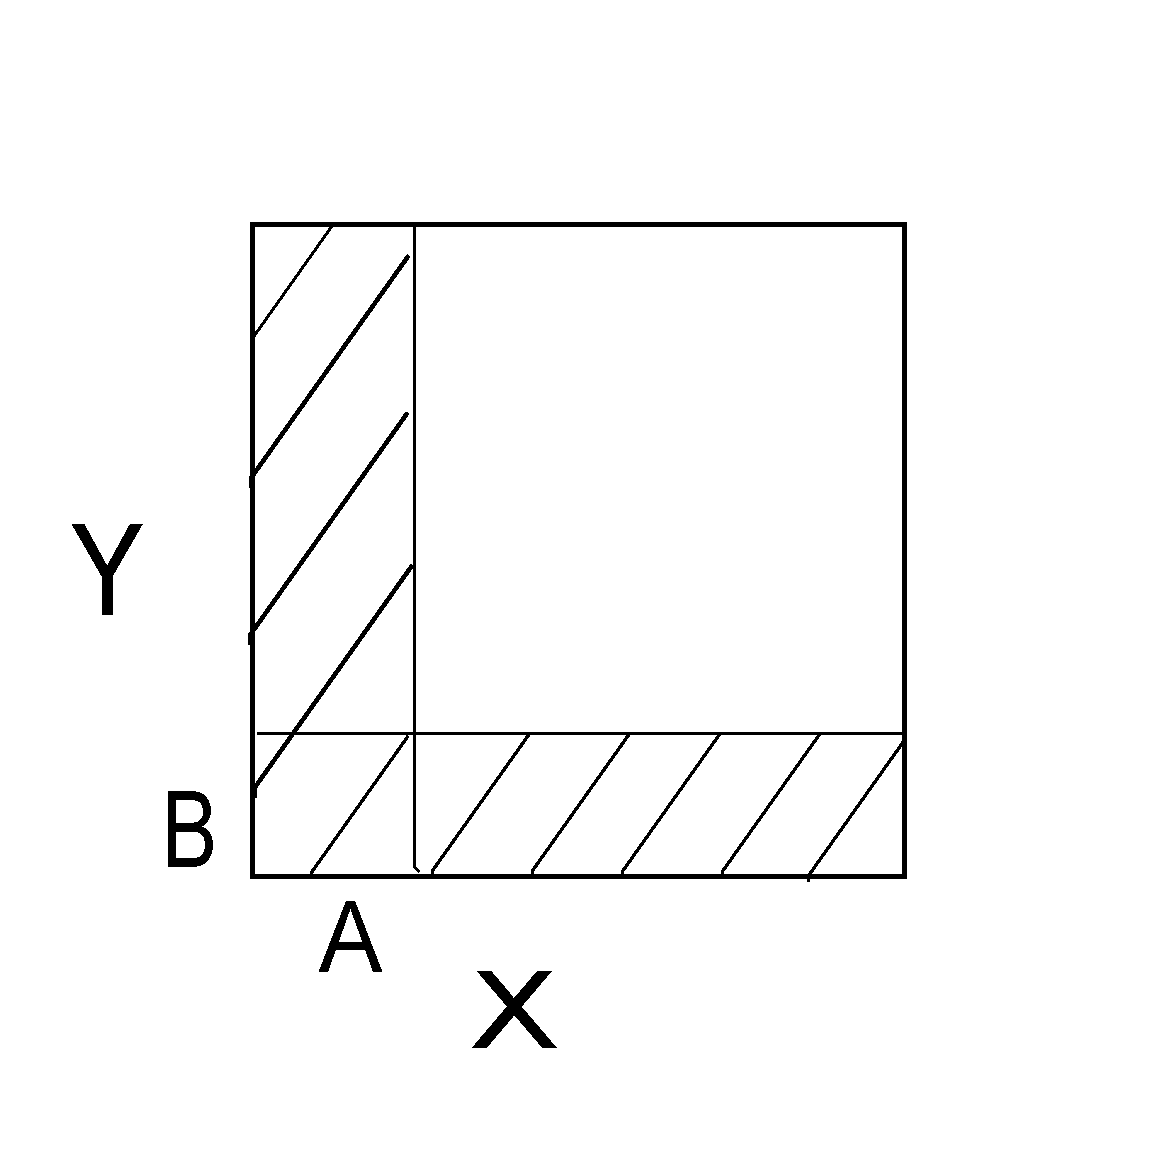
\includegraphics[width=0.2\textwidth]{figures/15.pdf}
\caption{\small Diagram of a relative product, for that last equality.}
\end{figure}

Now suppose $X = Y$; then we have a diagonal map $\Delta: (X, A \cup B) \to (X \times X, X \times B \cup A \times X)$ which induces a relative cup product:
\begin{ctikzcd}
K(X, A) \otimes K(X, B)\dar[equal] \rar["\smile"] & K(X, A \cup B) \\
\Ktwee(X/A) \otimes \Ktwee(X/B) \rar & K(X \times X, X \times B \cup A \times X)\uar["\Delta^*"]
\end{ctikzcd}
When $A \simeq \ptspace \simeq B$ we obtain
\begin{ctikzcd}
K(X, A) \otimes K(X, B)\dar[equal] \rar["\smile"] & \Ktwee(X,A\cup B)\rar &\Ktwee(X)\\
\Ktwee(X) \otimes \Ktwee(X) \rar & \Ktwee(X\sprod X)\uar["\Delta^*"]
\end{ctikzcd}
Where the map $\Ktwee(X,A\cup B)\to \Ktwee(X)$ is pulling back along the inclusion $(X,\ptspace)\to (X,A\cup B)$. This composite map $\Ktwee(X)\otimes \Ktwee(X)\to \Ktwee(X)$ is the product on reduced $K$ theory.
If in addition $A \cup B = X$, we get $K(X, A \cup B) = 0$, so the smash product map is trivial.  We have shown
\begin{lem}
If $X = A \cup B$ and $A \simeq \ptspace \simeq B$, then $\Ktwee(X)^2 = 0$; e.g., any suspension has this property.
\end{lem}
\begin{lem}
For all $n$, $K(S^{2n})=\Z[x_n]/x_n^2$, and $\psi^k(x_n)=k^nx_n.$
\end{lem}
\begin{proof}
\noindent By the previous lemma, $\Ktwee S^2 = \Z \langle \bundle{L} - 1 \rangle$ is subject to the relation $(\bundle{L} - 1)^2 = 0$.  So $K(S^2) = \Z[x_1]/x_1^2$. Now $\bundle{L}$ is a line bundle, so $\psi^k (\bundle{L}) = \bundle{L}^k$.  Thus
\[\psi^k(x)  = \psi^k(\bundle{L} - 1) = \bundle{L}^k - 1=(1+x_1)^k-1=kx_1.\]
By Bott, again, we have $\Ktwee(S^{2n}) \stackrel{\cong}{\from} \Ktwee(S^2)^{\otimes n}$, sending $x^{\otimes n}$ to $x_n=x_1^{\wedge n}$, so $K(S^{2n}) \cong \Z[x_n]/x_n^2$.

By lemma \ref{smashprodcommadams},
$\psi^k(x_n) = \psi^k(x_1^{\wedge n}) = \psi^k(x_1)^{\wedge n} = (kx_1)^{\wedge n} = k^n x_n$.
\end{proof}
\noindent
In particular, the Adams operations detect the dimension of an even-dimensional sphere!

\begin{wrapfigure}{r}{0.3\textwidth}
\centering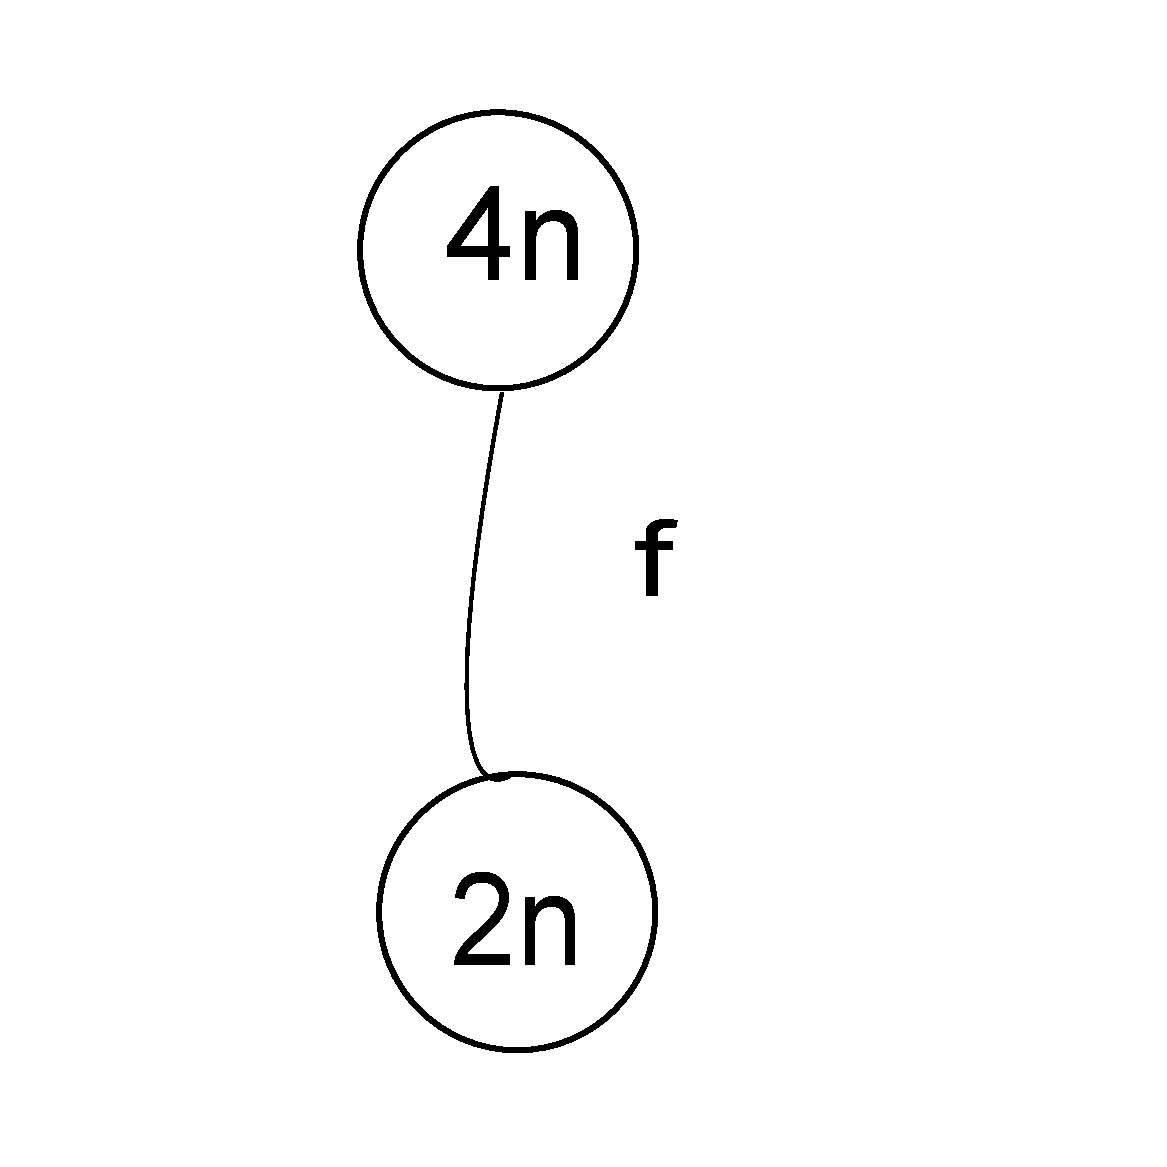
\includegraphics[width=0.2\textwidth]{figures/16.pdf}
\caption{\small Set-up for the Hopf invariant 1 problem.}
\end{wrapfigure}
OK, so now we can use all this equipment to prove that Hopf-invariant 1 problem. That is, we want to show that there is no element of Hopf invariant one in $\pi_{4n-1}(S^{2n})$ for $n\neq1,2,4$. Remember the set up:
\begin{ctikzcd}
S^{4n-1}\rar["f"] & S^{2n} \rar["i"] & X \rar["k"] & S^{4n}
\end{ctikzcd}
Here, $k$ is obtained by collapsing $X=C(f)$ onto its $4n$-cell, i.e.\ by continuing the cofiber sequence. As $f$ is 0 in $K$-theory, the long exact sequence obtained from the cofiber sequence $S^{2n}\to X\to S^{4n}$ degenerates into a short exact sequence of reduced $K$-groups, which splits $\Ktwee(X)$ into $\Z\langle x\rangle\oplus\Z\langle y\rangle$ (as $\Ktwee(S^{2n})$ is free):
\begin{ctikzcd}[row sep=0em]
0&\lar\Ktwee(S^{2n})&\lar["i^*"]\Ktwee(X)&\lar["j^*"]\Ktwee(S^{4n})&\lar0\\
 & x_n & \lar[mapsto]x \\
 && y  & \lar[mapsto] x_{2n}
\end{ctikzcd}
%So there is an $x \in \Ktwee(X)$ such that it pulls back to $x_n$.
Now $y^2=j^*(x_{2n})^2=0$, $i^*(x^2)=x_n^2=0$ and $i^*(xy)=x_n\cdot0=0$. Thus, for some $a,b\in\Z$, we have
\[K(X)=\Z\langle1,x,y\rangle\text{ with multiplication }y^2=0,\ x^2=ay,\ xy=by.\]
%In addition, $\Ktwee(X) \stackrel{j^*}{\from} \Ktwee(S^{4n})$ is injective, so $y^2 = j^* x_{2n}^2 = 0$.  This $K(X)$ has three generators, $\langle 1, x, y \rangle$, and the relations $y^2 = 0$, $x^2 = ay$.  ($x^2 = ay + bx$, but $b = 0$ since $0 = x_n^2 = i^* x^2 = b x_n$.)
\begin{claim}
$a$ is the Hopf invariant.
\end{claim}
\begin{proof}
There are a variety of ways to justify this claim; for example, you could use the Chern character, which provides a ring homomorphism $K(X) \to H^*(X; \Q)$.  Also the Atiyah-Hirzebruch spectral sequence works nicely: $E_2^{s, t} = H^s(X; K^t(\ptspace)) \Rightarrow K^*(X)$.  $X$ is very simple, so we can write this down easily:
\[E_2^{s,t}=0\text{ unless $t$ is even and $s=0,2n,4n$, otherwise $E_2^{s,t}\equiv\Z$.}\]
In particular, as every nonzero entry has even total dimension, there can be no differentials, and the spectral sequence collapses by $E_2$ page. In particular, we can identify the $E_2$ and $E_\infty$ pages.

Let $1\in H^{0}(X;K^0(\ptspace))$, $u\in H^{2n}(X;K^0(\ptspace))$ and $v\in H^{4n}(X;K^0(\ptspace))$ be generators. Then, if $p\in K^{-2}(\ptspace)$ is the periodicity element, $E_2^{2n,-2n}=\Z\langle p^nu\rangle$ and $E_2^{4n,-4n}=\Z\langle p^{2n}v\rangle$.
Now the total degree zero line computes $K(X)$, so that
\[K(X)=
\Z\langle1\rangle\oplus
\Z\langle p^nu\rangle\oplus
\Z\langle p^{2n}v\rangle\]
Now because the product on the $E_\infty$ page is induced by that on $K^*(X)$, we must have $(p^nu)\cdot(p^nu)=\pm a(p^{2n}v)$, and thus $u\cdot u=\pm av$. Finally, the product structure on $E_2^{*,0}$ is just the normal cup product structure of $H^*(X)$, showing that $a$ is the Hopf invariant.
%
%But everything in the $E_2$ term happens in even dimensions, so there are no differentials.  And since the spectral sequence is nice with respect to all the algebraic structure in sight, clearly the $x$ and $y$ represent the generators of $\Ktwee(X)$, and $a = H(f)$.
\end{proof}
\begin{thm}
The Hopf invariant $a$ cannot be odd unless $n = 1, 2, 4$.
\end{thm}
\begin{proof}
We'll start by assuming that $a$ is odd.
Firstly, for each $k$, $i^*(\psi^k(x))=\psi^k(x_n)=k^nx_n$. Moreover, $\psi^k(y)=\psi^k(j^*(x_{2n}))=j^*(\psi^kx_{2n})
=j^*(k^{2n}x_{2n})=k^{2n}y$. Thus, for some $b_k\in\Z$:
\[\psi^k(x)=k^nx+b_ky;\textup{ \ and \ }\psi^k(y)=k^{2n}y.\]
Now using lemma \ref{frobeniuslemma}, and writing $\equiv$ for congruence mod 2:
\[0\not\equiv ay=x^2\equiv\psi^2(x)=2^nx+b_2y.\]
Examining $y$ coefficients, we see that $b_2$ must be odd. Now we calculate:
\begin{align*}
\psi^3 \psi^2(x) & = \psi^3(2^n x + b_2 y) = 2^n(3^n x + b_3 y) + b_2 3^{2n} y, \\
\psi^2 \psi^3(x) & = \psi^2(3^n x + b_3 y) = 3^n(2^n x + b_2 y) + b_3 2^{2n} y.
\end{align*}
Again examining $y$ coefficients gives an equation $b_3(2^{2n} - 2^n) = b_2(3^{2n} - 3^n)$.  $2^n$ divides the left hand expression, and $b_2$ is odd, so $2^n$ must divide $3^n - 1$. The result follows from the next claim.
\end{proof}
\begin{claim}
$2^n$ can only divide $3^n - 1$ when $n=1,2,4$.
\end{claim}
\begin{proof}
Writing $\nu(m)$ for the largest number $r$ such that $2^r$ divides $m$, so that $2^n|3^n-1$ iff $\nu(3^n-1)\geq n$. If one can prove the following formula, the result is immediate:
\[
\nu(3^n-1) = \begin{cases} 1 & \hbox{$n$ odd}, \\ \nu(n) + 2 & \hbox{$n$ even}.\end{cases}
\]
To make this calculation, we have the following argument, due to David Anick. For any $e\geq0$:
\begin{alignat*}{3}
3^{2e+1} - 1 &= 9^e \cdot 3 - 1 &&\equiv 2 \pmod 8,\textup{ \ so that \ }&\nu(3^\textup{odd} - 1)&=1;\\
3^{2e+1} + 1 &= 9^e \cdot 3 + 1 &&\equiv 4 \pmod 8,\textup{ \ so that \ }&\nu(3^\textup{odd} + 1)&=2;\\
3^{2e} + 1 &= \ \ 9^e + 1 &&\equiv 2 \pmod 8,\textup{ \ so that \ }&\nu(3^\textup{even} + 1)&=1.
\end{alignat*}
If $n$ is odd, we are done. Else, write $n=2^{\nu(n)}d$ for $d$ odd, and factorise:
\[
3^n-1=3^{2^{\nu(n)} d} - 1 = (3^d + 1) (3^d - 1) (3^{2d} + 1) \cdots (3^{2^{{\nu(n)}-1}d} + 1).
\]
We count exactly $2+1+1+\cdots+1=\nu(n)+2$ factors of two in this expression, as advertised.
\end{proof}

% >>>
\fi
\begin{SummaryNote}
\Bullet In $K(X)$, $\psi^p(x) \equiv x^p \pmod{p}$  for $p$ prime.

\Bullet The dashed external smash product is induced by the solid vertical morphisms in the following diagram. It commutes with Adams operations. The lower short exact sequence appears because $X\vee Y\to X\times Y$ splits after one suspension.
\begin{ctikzcd}[column sep=small]
0\ar[r] & \Ktwee(X) \otimes \Ktwee(Y)\rar[r] \dar[dashed,"\wedge"]& K(X) \otimes K(Y)\rar["\alpha"]\dar["\times"]&\Ktwee(X) \oplus \Ktwee(Y) \oplus \Z\dar[equal]\rar&0\\
0\ar[r]&\Ktwee(X \sprod Y)\rar["c^*"]&K(X\times Y)\ar[r]&K(X\vee Y)\ar[r]&0
\end{ctikzcd}

\Bullet Products on $K(X)$ vanish if $X$ is the union of contractible subsets (e.g.\ $X=S^{n}$).

\Bullet  $K(S^{2})=\Z[x_1]/x_1^2$. Since $x_1+1$ is a line bundle, $\psi^k(x_1)=(x_1+1)^k-1=kx_1$.


\Bullet For all $n$, $K(S^{2n})=\Z[x_n]/x_n^2$, and $\psi^k(x_n)=k^nx_n$, as the smash product map commutes with $\psi^k$. Thus the Adams operations detect the $n$ in $S^{2n}$!%dimension of an even-dimensional sphere!

\Bullet This all comes together to prove Hopf invariant one.
\end{SummaryNote}
